\section{Registrar Module: Centralized Data Validation}
The Registrar office holds the authority for the final validation of applicant data before the admission is officially confirmed. 

\subsection{Master Applicant Queue}
The Registrar monitors the global applicant list to oversee the progress of the admission session across all faculties.

\begin{figure}[H]
    \centering
    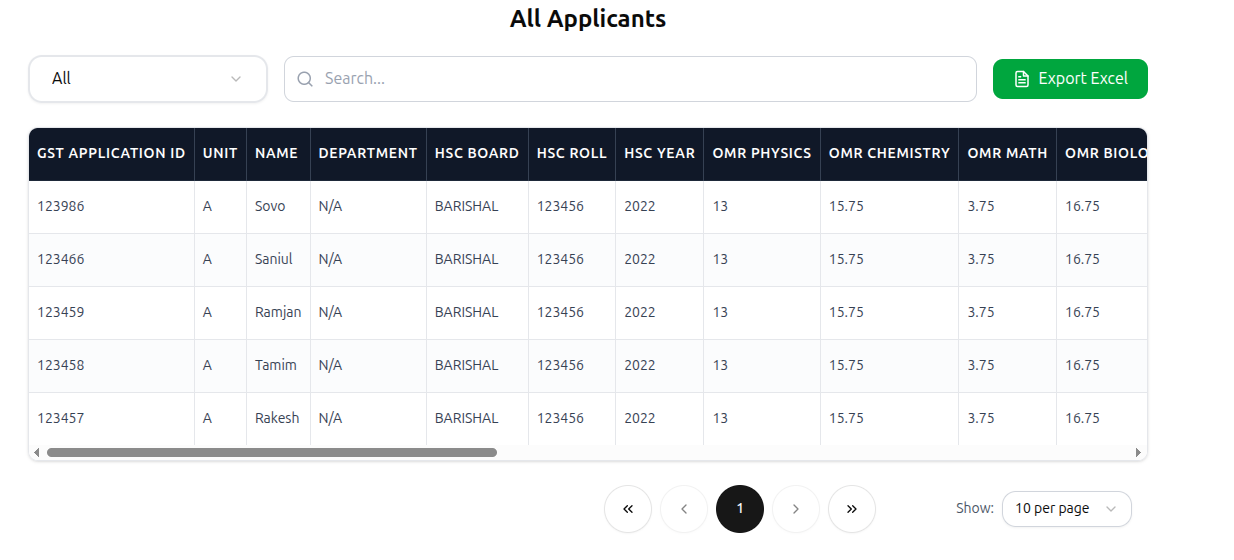
\includegraphics[width=0.9\textwidth]{chapters/chapter4/images/applicantList.png}
    \caption{Registrar's Master Applicant Data Interface}
    \label{fig:registrar_master_list}
\end{figure}

\subsection{Detailed Verification Matrix}
Using a more granular data table, the Registrar office cross-checks the physical document submission status with the digital records.

\begin{figure}[H]
    \centering
    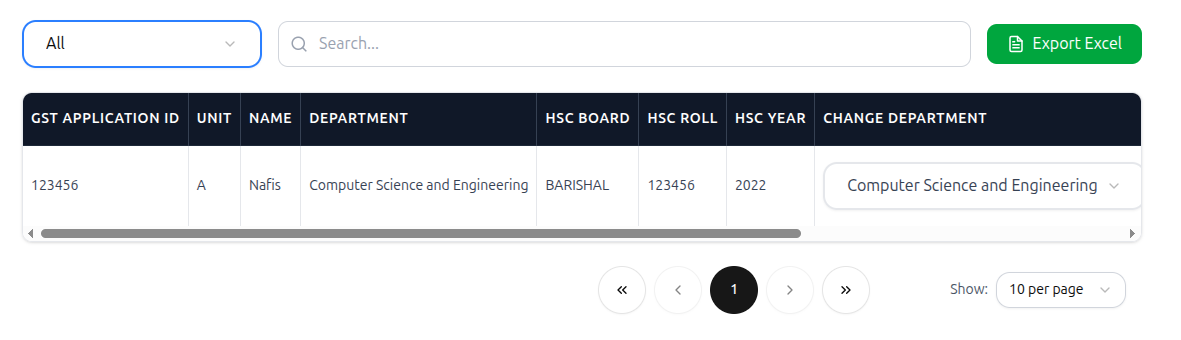
\includegraphics[width=0.9\textwidth]{chapters/chapter4/images/listTable.png}
    \caption{Registrar's Detailed Validation Table}
    \label{fig:registrar_table_view}
\end{figure}

This dual-layer verification ensures that only students with legitimate academic credentials and fee payments are processed for the final step.